\documentclass[10pt]{beamer}
\usepackage[T1]{fontenc}
\usepackage[utf8]{inputenc}
\usepackage[french]{babel}
\usepackage{color}
\usepackage[normalem]{ ulem }
\usepackage{soul}
\usetheme{Darmstadt}

\begin{document}
\begin{frame}{Matériels SAVOIE}
\begin{block}{Quatre ESX}
\begin{itemize}
\item DELL R430 Intel Xeon E5 2.4GHz
\item 32GB de RAM 
\item 2 disques durs de 300GB en RAID 1
\item 4x1 GB Ethernet et une carte 4 ports 1 GB additionnelle
\end{itemize}
\end{block}
\begin{block}{Deux SAN}
\begin{itemize}
\item Synology RS818RP+
\item 4 disques durs Seagate Barracuda 6 To
\item Alimentation redondée
\end{itemize}
\end{block}
\end{frame}

\begin{frame}{Composition matérielle de la plate-forme}
\begin{block}{Sur le segment OPS}
\begin{itemize}
\item 4 ESX : lesmenuires.ops, valthorens.ops, meribel.ops et courchevel.ops
\item 2 SAN : lachambre.ops et saulire.ops
\item 1 station d'administration : latania.ops
\end{itemize}
\end{block}
\begin{block}{Sur le segment PREOPS}
\begin{itemize}
\item 3 ESX : valthorens.preops, meribel.preops et courchevel.preops
\item 2 SAN : lachambre.preops et saulire.preops
\item 1 station d'administration : latania.preops
\end{itemize}
\end{block}
\end{frame}

\begin{frame}{Adressage réseaux}
\begin{center}
\begin{tabular}{|l|c|r|}
  \hline
  colonne 1 & colonne 2 & colonne 3 \\
  \hline
  1.1 & 1.2 & 1.3 \\
  2.1 & 2.2 & 2.3 \\
  \hline
\end{tabular}
\end{center}
\end{frame}

\begin{center}
\begin{frame}{Comment le stockage est-il conceptualisé dans SAVOIE ?}
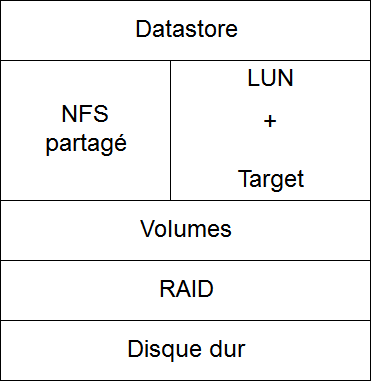
\includegraphics[width=200px]{Concepts_Stockage.png}
\end{frame}
\end{center}









\begin{frame}{RAID 10}
\begin{block}{Fonctionnement}
\begin{itemize}
\item 2 disques en RAID0 : répartir les informations stockées sur plusieurs disques durs grâce à un entrelacement des données. Temps d'accès accéléré.
\item 2 disques en RAID1 : l’un est utilisé en miroir de l'autre
\end{itemize}
\end{block}
\begin{block}{Avantages et inconvénients}
\begin{itemize}
\item Permet la performance et la disponibilité
\item Performance de 50\% (4*6To=>12To)
\end{itemize}
\end{block}
\end{frame}

 
\begin{frame}{Un langage particulier}
\begin{block}{Vocabulaire de base}
\begin{itemize}
\item ESX, ESXi, hôte, noeud, serveurs
\item Hyperviseur, VSphere
\item VM, MV
\end{itemize}  
\end{block} 

\end{frame}



\begin{frame}{vCenter}
\begin{block}{}
\begin{itemize}
\item Interface Web permettant de gérer un inventaire d’objets VMware de manière homogène et conviviale
\item Le vCenter est lui-même une VM que l’on déploie sur un ESX. On peut donc lui appliquer les mécanismes de HA de VMWare (vMotion, HA, FT)
\item Le vCenter permet de déployer de manière optimale les patchs de sécurité sur chaque ESX et sur vCenter lui-même
\item Nécessité de sauvegarder la configuration d’un vCenter de plus en plus critique
\end{itemize}
\end{block}
\end{frame}

\begin{frame}{Choix de l'hyperviseur}
\begin{block}{Avantages}
\begin{itemize}
\item Leader du marché, gage de pérennité et de solidité
\item Facilité pour trouver un prestataire de formation
\item Solution complète au-delà de vSphere et vCenter (vCloud, vRealize, API SVG, etc)
\item Régularité et réactivité au niveau des patchs et solutions de sécurité
\item Interfaces graphiques conviviales et puissantes (Clickodrome)
\item Expérience de Clément au travers de sa QTS et des ESX-TLC
\end{itemize}
\end{block}
\begin{block}{Inconvénients}
\begin{itemize}
\item Coût financier important à rentabiliser
\begin{itemize}
    \item Dès lors que le nombre d’applications hébergées est important
\item Dès lors que le choix des licences est judicieux
\end{itemize}
\item Coût RH important rentabilisé dès lors qu’on arrête d’installer N services identiques pour N projets 
\end{itemize}
\end{block}
\end{frame}

\begin{frame}{Qu'est ce qu'une VM ?}
\begin{block}{Une VM est un ensemble de fichiers}
\begin{itemize}
\item \textbf{.VMDK} : Disque dur virtuel VMware.
\item \textbf{.VMX }: Fichier de configuration de la machine virtuelle. Contient toutes les informations que vous paramétrez via l’interface graphique du logiciel. Exemples : nom de la machine, type d’OS, RAM, carte réseau, type de connexion,…
\item \textbf{.VWSP} : Fichier d’échange (correspond au SWAP).
\item \textbf{.VMSS} : Fichier qui enregistre l’état de la VM lorsqu’elle est suspendue (ce qui permet la reprise par la suite).
\item \textbf{.NVRAM} : Fichier correspondant au BIOS de la VM  
\item \textbf{.VMSN} : Contient l'état de la machine quand vous faite un snapshot (en créant un fichier par snapshot).
\item \textbf{.LOG} : Enregistre les logs sur ce qu'il se passe sur la VM. 
\end{itemize}
\end{block} 
\end{frame}

\begin{center}
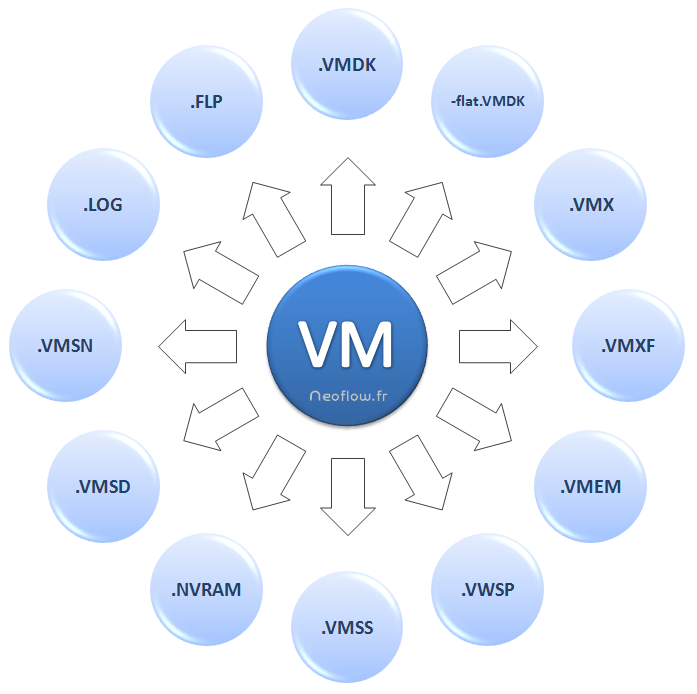
\includegraphics[width=230px]{filevm.png}   
\end{center}

\end{document}



 